% Created by tikzDevice version 0.10.1 on 2017-03-15 16:22:58
% !TEX encoding = UTF-8 Unicode
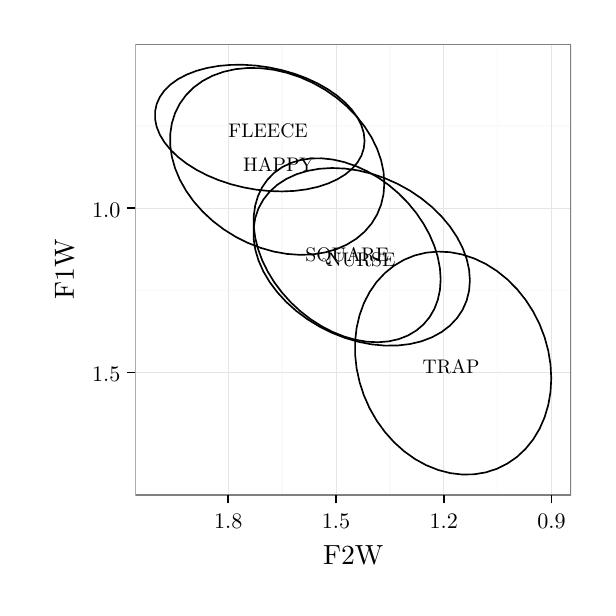
\begin{tikzpicture}[x=1pt,y=1pt]
\definecolor{fillColor}{RGB}{255,255,255}
\path[use as bounding box,fill=fillColor,fill opacity=0.00] (0,0) rectangle (202.36,202.36);
\begin{scope}
\path[clip] (  0.00,  0.00) rectangle (202.36,202.36);
\definecolor{drawColor}{RGB}{255,255,255}
\definecolor{fillColor}{RGB}{255,255,255}

\path[draw=drawColor,line width= 0.6pt,line join=round,line cap=round,fill=fillColor] (  0.00,  0.00) rectangle (202.36,202.36);
\end{scope}
\begin{scope}
\path[clip] ( 38.88, 33.48) rectangle (196.36,196.36);
\definecolor{fillColor}{RGB}{255,255,255}

\path[fill=fillColor] ( 38.88, 33.48) rectangle (196.36,196.36);
\definecolor{drawColor}{gray}{0.98}

\path[draw=drawColor,line width= 0.6pt,line join=round] ( 38.88,166.79) --
	(196.36,166.79);

\path[draw=drawColor,line width= 0.6pt,line join=round] ( 38.88,107.43) --
	(196.36,107.43);

\path[draw=drawColor,line width= 0.6pt,line join=round] (169.81, 33.48) --
	(169.81,196.36);

\path[draw=drawColor,line width= 0.6pt,line join=round] (130.89, 33.48) --
	(130.89,196.36);

\path[draw=drawColor,line width= 0.6pt,line join=round] ( 91.97, 33.48) --
	( 91.97,196.36);
\definecolor{drawColor}{gray}{0.90}

\path[draw=drawColor,line width= 0.2pt,line join=round] ( 38.88,137.11) --
	(196.36,137.11);

\path[draw=drawColor,line width= 0.2pt,line join=round] ( 38.88, 77.75) --
	(196.36, 77.75);

\path[draw=drawColor,line width= 0.2pt,line join=round] (189.27, 33.48) --
	(189.27,196.36);

\path[draw=drawColor,line width= 0.2pt,line join=round] (150.35, 33.48) --
	(150.35,196.36);

\path[draw=drawColor,line width= 0.2pt,line join=round] (111.43, 33.48) --
	(111.43,196.36);

\path[draw=drawColor,line width= 0.2pt,line join=round] ( 72.50, 33.48) --
	( 72.50,196.36);
\definecolor{drawColor}{RGB}{0,0,0}

\node[text=drawColor,anchor=base,inner sep=0pt, outer sep=0pt, scale=  0.71] at ( 86.89,162.51) {FLEECE};

\node[text=drawColor,anchor=base,inner sep=0pt, outer sep=0pt, scale=  0.71] at ( 90.71,150.28) {HAPPY};

\node[text=drawColor,anchor=base,inner sep=0pt, outer sep=0pt, scale=  0.71] at (120.57,116.10) {NURSE};

\node[text=drawColor,anchor=base,inner sep=0pt, outer sep=0pt, scale=  0.71] at (115.47,117.90) {SQUARE};

\node[text=drawColor,anchor=base,inner sep=0pt, outer sep=0pt, scale=  0.71] at (153.00, 77.50) {TRAP};

\path[draw=drawColor,line width= 0.6pt,line join=round] (121.74,161.44) --
	(121.45,164.23) --
	(120.60,167.05) --
	(119.18,169.85) --
	(117.23,172.60) --
	(114.78,175.25) --
	(111.85,177.76) --
	(108.50,180.09) --
	(104.78,182.21) --
	(100.74,184.09) --
	( 96.44,185.69) --
	( 91.96,186.99) --
	( 87.35,187.98) --
	( 82.69,188.64) --
	( 78.04,188.95) --
	( 73.48,188.92) --
	( 69.08,188.54) --
	( 64.91,187.82) --
	( 61.02,186.77) --
	( 57.48,185.41) --
	( 54.33,183.75) --
	( 51.64,181.83) --
	( 49.43,179.67) --
	( 47.75,177.30) --
	( 46.61,174.76) --
	( 46.04,172.09) --
	( 46.04,169.33) --
	( 46.61,166.52) --
	( 47.75,163.70) --
	( 49.43,160.92) --
	( 51.64,158.22) --
	( 54.33,155.63) --
	( 57.48,153.21) --
	( 61.02,150.98) --
	( 64.91,148.98) --
	( 69.08,147.23) --
	( 73.48,145.78) --
	( 78.04,144.63) --
	( 82.69,143.80) --
	( 87.35,143.32) --
	( 91.96,143.18) --
	( 96.44,143.38) --
	(100.74,143.93) --
	(104.78,144.82) --
	(108.50,146.03) --
	(111.85,147.54) --
	(114.78,149.33) --
	(117.23,151.38) --
	(119.18,153.65) --
	(120.60,156.11) --
	(121.45,158.72) --
	(121.74,161.44);

\path[draw=drawColor,line width= 0.6pt,line join=round] (128.88,146.19) --
	(128.59,150.29) --
	(127.71,154.44) --
	(126.27,158.59) --
	(124.28,162.67) --
	(121.77,166.62) --
	(118.78,170.38) --
	(115.35,173.89) --
	(111.55,177.10) --
	(107.42,179.96) --
	(103.03,182.42) --
	( 98.45,184.46) --
	( 93.73,186.04) --
	( 88.97,187.13) --
	( 84.22,187.72) --
	( 79.57,187.80) --
	( 75.07,187.36) --
	( 70.80,186.42) --
	( 66.83,185.00) --
	( 63.21,183.10) --
	( 59.99,180.76) --
	( 57.24,178.02) --
	( 54.98,174.91) --
	( 53.26,171.49) --
	( 52.10,167.80) --
	( 51.51,163.90) --
	( 51.51,159.86) --
	( 52.10,155.72) --
	( 53.26,151.56) --
	( 54.98,147.44) --
	( 57.24,143.42) --
	( 59.99,139.56) --
	( 63.21,135.92) --
	( 66.83,132.55) --
	( 70.80,129.51) --
	( 75.07,126.84) --
	( 79.57,124.59) --
	( 84.22,122.78) --
	( 88.97,121.44) --
	( 93.73,120.60) --
	( 98.45,120.26) --
	(103.03,120.44) --
	(107.42,121.13) --
	(111.55,122.31) --
	(115.35,123.98) --
	(118.78,126.10) --
	(121.77,128.65) --
	(124.28,131.58) --
	(126.27,134.85) --
	(127.71,138.41) --
	(128.59,142.21) --
	(128.88,146.19);

\path[draw=drawColor,line width= 0.6pt,line join=round] (159.80,111.03) --
	(159.50,114.90) --
	(158.62,118.84) --
	(157.16,122.79) --
	(155.14,126.70) --
	(152.61,130.49) --
	(149.59,134.11) --
	(146.13,137.52) --
	(142.29,140.65) --
	(138.12,143.47) --
	(133.68,145.92) --
	(129.05,147.97) --
	(124.29,149.59) --
	(119.48,150.75) --
	(114.68,151.44) --
	(109.97,151.65) --
	(105.43,151.37) --
	(101.12,150.61) --
	( 97.11,149.38) --
	( 93.45,147.69) --
	( 90.20,145.58) --
	( 87.42,143.07) --
	( 85.14,140.21) --
	( 83.40,137.03) --
	( 82.23,133.59) --
	( 81.64,129.93) --
	( 81.64,126.12) --
	( 82.23,122.21) --
	( 83.40,118.26) --
	( 85.14,114.32) --
	( 87.42,110.47) --
	( 90.20,106.75) --
	( 93.45,103.23) --
	( 97.11, 99.95) --
	(101.12, 96.98) --
	(105.43, 94.34) --
	(109.97, 92.08) --
	(114.68, 90.25) --
	(119.48, 88.85) --
	(124.29, 87.92) --
	(129.05, 87.47) --
	(133.68, 87.51) --
	(138.12, 88.03) --
	(142.29, 89.03) --
	(146.13, 90.49) --
	(149.59, 92.39) --
	(152.61, 94.71) --
	(155.14, 97.40) --
	(157.16,100.42) --
	(158.62,103.74) --
	(159.50,107.29) --
	(159.80,111.03);

\path[draw=drawColor,line width= 0.6pt,line join=round] (149.23,111.39) --
	(148.97,115.35) --
	(148.21,119.41) --
	(146.95,123.50) --
	(145.21,127.57) --
	(143.02,131.55) --
	(140.41,135.39) --
	(137.42,139.03) --
	(134.10,142.40) --
	(130.50,145.47) --
	(126.67,148.18) --
	(122.66,150.49) --
	(118.55,152.37) --
	(114.39,153.78) --
	(110.25,154.72) --
	(106.19,155.15) --
	(102.26,155.09) --
	( 98.54,154.52) --
	( 95.07,153.46) --
	( 91.91,151.92) --
	( 89.10,149.92) --
	( 86.70,147.50) --
	( 84.73,144.69) --
	( 83.23,141.54) --
	( 82.21,138.09) --
	( 81.70,134.40) --
	( 81.70,130.52) --
	( 82.21,126.50) --
	( 83.23,122.42) --
	( 84.73,118.33) --
	( 86.70,114.30) --
	( 89.10,110.38) --
	( 91.91,106.63) --
	( 95.07,103.12) --
	( 98.54, 99.89) --
	(102.26, 97.00) --
	(106.19, 94.49) --
	(110.25, 92.39) --
	(114.39, 90.74) --
	(118.55, 89.56) --
	(122.66, 88.87) --
	(126.67, 88.69) --
	(130.50, 89.01) --
	(134.10, 89.82) --
	(137.42, 91.13) --
	(140.41, 92.90) --
	(143.02, 95.11) --
	(145.21, 97.73) --
	(146.95,100.71) --
	(148.21,104.02) --
	(148.97,107.60) --
	(149.23,111.39);

\path[draw=drawColor,line width= 0.6pt,line join=round] (189.20, 75.65) --
	(188.93, 80.60) --
	(188.13, 85.56) --
	(186.80, 90.45) --
	(184.98, 95.20) --
	(182.68, 99.74) --
	(179.94,103.99) --
	(176.81,107.90) --
	(173.32,111.40) --
	(169.54,114.45) --
	(165.52,116.99) --
	(161.32,118.98) --
	(157.00,120.41) --
	(152.64,121.23) --
	(148.29,121.45) --
	(144.02,121.06) --
	(139.90,120.07) --
	(135.99,118.48) --
	(132.35,116.33) --
	(129.04,113.65) --
	(126.09,110.47) --
	(123.57,106.85) --
	(121.50,102.84) --
	(119.93, 98.50) --
	(118.86, 93.89) --
	(118.32, 89.10) --
	(118.32, 84.18) --
	(118.86, 79.22) --
	(119.93, 74.29) --
	(121.50, 69.46) --
	(123.57, 64.80) --
	(126.09, 60.40) --
	(129.04, 56.31) --
	(132.35, 52.60) --
	(135.99, 49.32) --
	(139.90, 46.52) --
	(144.02, 44.25) --
	(148.29, 42.54) --
	(152.64, 41.41) --
	(157.00, 40.88) --
	(161.32, 40.97) --
	(165.52, 41.66) --
	(169.54, 42.96) --
	(173.32, 44.83) --
	(176.81, 47.25) --
	(179.94, 50.19) --
	(182.68, 53.59) --
	(184.98, 57.42) --
	(186.80, 61.60) --
	(188.13, 66.08) --
	(188.93, 70.79) --
	(189.20, 75.65);
\definecolor{drawColor}{gray}{0.50}

\path[draw=drawColor,line width= 0.6pt,line join=round,line cap=round] ( 38.88, 33.48) rectangle (196.36,196.36);
\end{scope}
\begin{scope}
\path[clip] (  0.00,  0.00) rectangle (202.36,202.36);
\definecolor{drawColor}{RGB}{0,0,0}

\node[text=drawColor,anchor=base east,inner sep=0pt, outer sep=0pt, scale=  0.80] at ( 33.48,133.80) {1.0};

\node[text=drawColor,anchor=base east,inner sep=0pt, outer sep=0pt, scale=  0.80] at ( 33.48, 74.44) {1.5};
\end{scope}
\begin{scope}
\path[clip] (  0.00,  0.00) rectangle (202.36,202.36);
\definecolor{drawColor}{RGB}{0,0,0}

\path[draw=drawColor,line width= 0.6pt,line join=round] ( 35.88,137.11) --
	( 38.88,137.11);

\path[draw=drawColor,line width= 0.6pt,line join=round] ( 35.88, 77.75) --
	( 38.88, 77.75);
\end{scope}
\begin{scope}
\path[clip] (  0.00,  0.00) rectangle (202.36,202.36);
\definecolor{drawColor}{RGB}{0,0,0}

\path[draw=drawColor,line width= 0.6pt,line join=round] (189.27, 30.48) --
	(189.27, 33.48);

\path[draw=drawColor,line width= 0.6pt,line join=round] (150.35, 30.48) --
	(150.35, 33.48);

\path[draw=drawColor,line width= 0.6pt,line join=round] (111.43, 30.48) --
	(111.43, 33.48);

\path[draw=drawColor,line width= 0.6pt,line join=round] ( 72.50, 30.48) --
	( 72.50, 33.48);
\end{scope}
\begin{scope}
\path[clip] (  0.00,  0.00) rectangle (202.36,202.36);
\definecolor{drawColor}{RGB}{0,0,0}

\node[text=drawColor,anchor=base,inner sep=0pt, outer sep=0pt, scale=  0.80] at (189.27, 21.47) {0.9};

\node[text=drawColor,anchor=base,inner sep=0pt, outer sep=0pt, scale=  0.80] at (150.35, 21.47) {1.2};

\node[text=drawColor,anchor=base,inner sep=0pt, outer sep=0pt, scale=  0.80] at (111.43, 21.47) {1.5};

\node[text=drawColor,anchor=base,inner sep=0pt, outer sep=0pt, scale=  0.80] at ( 72.50, 21.47) {1.8};
\end{scope}
\begin{scope}
\path[clip] (  0.00,  0.00) rectangle (202.36,202.36);
\definecolor{drawColor}{RGB}{0,0,0}

\node[text=drawColor,anchor=base,inner sep=0pt, outer sep=0pt, scale=  1.00] at (117.62,  8.40) {F2W};
\end{scope}
\begin{scope}
\path[clip] (  0.00,  0.00) rectangle (202.36,202.36);
\definecolor{drawColor}{RGB}{0,0,0}

\node[text=drawColor,rotate= 90.00,anchor=base,inner sep=0pt, outer sep=0pt, scale=  1.00] at ( 16.67,114.92) {F1W};
\end{scope}
\end{tikzpicture}
